
\documentclass[12pt]{article}
\usepackage{txfonts}
\usepackage{graphicx}
\usepackage{mygb4e}
\usepackage{solution}

\hidesolutions
\setlength\oddsidemargin{0.01in}
\setlength\topmargin{-1in}
\setlength\textwidth{6.9in}
\setlength\textheight{9.5in} 

\newcommand{\nl}{\mbox{$\langle cr \rangle$}}
\newcommand{\decaf}{\mbox{\textbf{\texttt{Decaf}}}}
\newcommand{\kw}[1]{\textbf{#1}}
\newcommand{\ident}[1]{\texttt{#1}}
\newcommand{\nonterm}[1]{\mbox{$\langle\mbox{#1}\rangle$\ }}
\newcommand{\term}[1]{\mbox{\textbf{#1}\ }}
\newcommand{\termchar}[1]{\mbox{\textbf{`\texttt{#1}'}\ }}
\newcommand{\once}[1]{\mbox{$\Big[\mbox{#1}\Big]$\ }}
\newcommand{\kstar}[1]{\mbox{\mbox{#1}$^\ast$\ }}
\newcommand{\plus}[1]{\mbox{\mbox{#1}$^+$\ }}
\newcommand{\leftgroup}{\mbox{\textbf{\Big\{}\ }}
\newcommand{\rightgroup}{\mbox{\textbf{\Big\}\ }}}
\newcommand{\group}[1]{\mbox{\leftgroup\ #1\ \rightgroup}\ }
\newcommand{\charconst}[1]{'\texttt{#1}'\ }
\newcommand{\sep}{\mbox{$\mid$}\ \ }
\newcommand{\commasep}[1]{\mbox{\leftgroup\mbox{#1}\rightgroup$^+$\textbf{,}}\ }
\newcommand{\cfgrule}[2]{#1 & \rightarrow & #2 \nonumber}

\raggedright

\newcommand{\valueof}[1]{\lbrack\!\lbrack #1 \rbrack\!\rbrack}
\newcommand{\refp}[1]{(\protect\ref{#1})}
\def\rwd#1 {\mbox{#1}}
\def\N{\ensuremath{\mathcal{N}}}
\def\implies{\ensuremath{\Rightarrow}}
% Set some text inside an fbox the full width of the line, with the frame
% sticking out into the margin.
\long\def\framepar#1{\par\noindent\hbox to \textwidth {\hskip-\fboxsep
\fbox{\parbox{\the\textwidth}{#1}}}}

\begin{document}
%\setlength{\baselineskip}{12pt}

\begin{center}
{\Large\bf
CMPT 379 - Sample Questions for Final Exam Preparation}\\
\end{center}

\bigskip

\begin{exe}


\ex\label{cfg} Regular and Context-free Grammars:

\begin{xlist}

{\ex Consider the following DFA:

\begin{center}
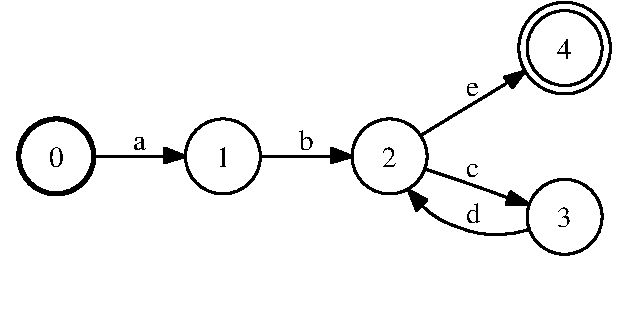
\includegraphics[width=3.5in]{figures/quiz1-dfa1}
\end{center}

Provide a regular expression for the regular language generated by this DFA.

\begin{soln}
\texttt{ab(cd)*e}
\end{soln}
}

{\ex You are given the following ordered list of token 
definitions:
\begin{tabbing}
123456789\=\kill
{\tt TOKEN\_A} \> $(ab)^\ast a$ \\
{\tt TOKEN\_B} \> $(ab)^\ast a (ca)^\ast$ \\
{\tt TOKEN\_C} \> $bab(bab)^\ast$ \\
{\tt TOKEN\_D} \> $a^\ast ba(ba)^\ast$
\end{tabbing}

Provide the tokenized output for the input string {\em abacabababa} using
the greedy longest match lexical analysis method.
\begin{soln}
\par\noindent First match:
\begin{tabbing}
123456789\=\kill
{\tt TOKEN\_A} \> $aba$ \\
{\tt TOKEN\_B} \> $abaca$ \\
{\tt TOKEN\_C} \> \textrm{no match} \\
{\tt TOKEN\_D} \> $aba$ 
\end{tabbing}

\par\noindent Second match:
\begin{tabbing}
123456789\=\kill
{\tt TOKEN\_A} \> \textrm{no match} \\
{\tt TOKEN\_B} \> \textrm{no match} \\
{\tt TOKEN\_C} \> $bab$ \\
{\tt TOKEN\_D} \> $bababa$ 
\end{tabbing}

\par\noindent Output:
\begin{tabbing}
123456789\=\kill
{\tt TOKEN\_B} \> $abaca$ \\
{\tt TOKEN\_D} \> $bababa$ 
\end{tabbing}
\end{soln}
}

{\ex The following CFG generates a regular language.
Provide a regular expression that generates the same language as this CFG.
\begin{eqnarray}
S & \rightarrow & AB \nonumber \\
A & \rightarrow & c \mid \epsilon \nonumber \\
B & \rightarrow & cbB \mid ca \nonumber
\end{eqnarray}

\begin{soln}
\begin{verbatim}
c?(cb)*ca
\end{verbatim}
\end{soln}
}

{\ex Are the following two context-free grammars equivalent? That is, 
do the two grammars generate the same language. Give a short precise
reason for your answer.
\begin{minipage}[t]{3in}
\begin{eqnarray}
G_1: && \nonumber \\
S & \rightarrow & AB \nonumber \\
A & \rightarrow & c \mid \epsilon \nonumber \\
B & \rightarrow & cbB \mid ca \nonumber
\end{eqnarray}
\end{minipage}
\begin{minipage}[t]{3in}
\begin{eqnarray}
G_2: && \nonumber \\
S & \rightarrow & cAa \nonumber \\
A & \rightarrow & cB \mid B \nonumber \\
B & \rightarrow & bcB \mid \epsilon \nonumber
\end{eqnarray}
\end{minipage}

\bigskip
\begin{soln}
\begin{verbatim}
c?(cb)*ca
\end{verbatim}
is equivalent to
\begin{verbatim}
cc?(bc)*a
\end{verbatim}
\end{soln}

}

{\ex Each of the following C code fragments has a lexical or syntax error (or warning), or both. 
For each example, indicate if the compiler would generate a {\em lexical} and/or {\em syntax} error
(or warning).

\begin{enumerate}

\item {\small\tt void main() \{ char c = 'ab';  \}} 
\begin{soln}
lexical error/warning: multi-character character constant
\end{soln}

\item {\small\tt void main() \{ char a[] = "ab ; \}}
\begin{soln}

\noindent
lexical error: missing terminating " character \\
syntax error: parse error at end of input
\end{soln}

\item {\small\tt void main() \{ int x = 3 int y = 4; \}}
\begin{soln}
syntax error: parse error before 'int'
\end{soln}

\item {\small\tt void main() \{ intx = 3; \}}
\begin{soln}
syntax error (symbol table error): 'intx' undeclared
\end{soln}

\item {\small\tt void main() \{ char a[] = "ab; printf("$\backslash$n"); \}}
\begin{soln}

\noindent
syntax error: parse error before 'n' \\
lexical error: missing terminating " character
\end{soln}

\end{enumerate}

}
\end{xlist}

\newpage

   \ex\label{derivative} 
   For alphabet $\Sigma$ let us denote the {\em derivative} of a regular expression
   $R$ with respect to $a$, where $a \in \Sigma$ as $\frac{dR}{da}$ or equivalently as
   $D_a[R]$. For any regular expression $R$, $D_a[R]$ is defined recursively using the following rules:
   	\begin{eqnarray}
		D_a[a] & = & \epsilon \label{e1} \\
		D_a[b] & = & \phi \textrm{,\ for $b \in \Sigma$, $b \neq a$, or $b = \epsilon$ or $b = \phi$}
			\label{e2}
	\end{eqnarray}
    If $P$ and $Q$ are regular expressions, then:
   \begin{eqnarray}
   D_a[P \mid Q] & = & D_a[P] \mid D_a[Q] \label{e3} \\
   D_a[P Q] & = & D_a[P] Q \mid \delta(P) D_a[Q] \label{e4} \\
   D_a[P^\ast] & = & D_a[P] P^\ast \label{e5}
   \end{eqnarray}
   where $\delta(P) = \epsilon$, if $\epsilon \in P$ and $\delta(P) = \phi$, if $\epsilon \not\in P$.

   The empty set $\phi$, is different from the empty string $\epsilon$, and has the following properties:
   \[ \begin{array}{lllll}
   \phi \mid R & = & R \mid \phi & = & R \\
   \phi R & = & R \phi & = & \phi
   \end{array} \]
   Also, we define derivative $D_s[R]$ of regular expression $R$ with respect to a sequence of symbols $s = a_1, a_2, \ldots, a_r$ as:
   \[ D_s[R] = D_{a_1, \ldots, a_r}[R] = D_{a_r}[ D_{a_1, \ldots, a_{r-1}}[R] ] \]
    A sequence $s$ of zero length is written as: $D_\epsilon[R] = R$.
    
   The intuition behind the notion of a derivative of a regular expression 
   $R$ with respect to symbol $a$ is that it provides
   us with a regular expression $R'$ such that the language of $R'$, 
   $L_{R'} = \{ y \mid ay \in L_R \}$.
   
   Let $R = (0 \mid 1)^\ast 1$, the derivative $D_a[R]$ for any symbol $a \in \Sigma$, 
   where $\Sigma = \{0,1\}$ is:
   \begin{eqnarray}
   D_a[R] & = & D_a[ (0 \mid 1)^\ast 1 ] \nonumber \\
   & = & D_a[ (0 \mid 1)^\ast ]\ 1 \mid D_a[ 1 ] \textrm{,\ since $\epsilon \in (0 \mid 1)^\ast$} 
   \textrm{\ \ \ using~(\ref{e4})} \nonumber \\
   & = & D_a[ 0 \mid 1 ]\ (0 \mid 1)^\ast\ 1 \mid D_a[ 1 ] 
   \textrm{\ \ \ using~(\ref{e5})} \nonumber \\
   & = & ( D_a[0] \mid D_a[1] )\ (0 \mid 1)^\ast\ 1 \mid D_a[1] 
   \textrm{\ \ \ using~(\ref{e3})} \nonumber
   \end{eqnarray}
   Putting in $a = 0$, we get:
   \begin{eqnarray}
   D_0[R] & = & (\epsilon \mid \phi) (0 \mid 1)^\ast 1 \mid \phi 
   \textrm{\ \ \ using~(\ref{e1}) and~(\ref{e2})} \nonumber
   %%D_1[R] & = & (\phi \mid \epsilon) (0 \mid 1)^\ast 1 \mid \epsilon \nonumber
   \end{eqnarray}
   This expressions can be simplified with identities for $\epsilon$ and $\phi$ to get:
   \[ \begin{array}{lllll}
   D_0[R] & = & (0 \mid 1)^\ast 1 & = & R
   %%D_1[R] & = & (0 \mid 1)^\ast 1 \mid \epsilon & = & R \mid \epsilon
   \end{array} \]
   We know from our previous definition that $D_\epsilon[R] = R = D_0[R]$. 
   Provide the simplified expressions for the following derivatives of $R = (0 \mid 1)^\ast 1$:
   
   \begin{xlist}
   
   \item $D_1[R]$
   \begin{soln}
   \[ D_1[R] = (\phi \mid \epsilon) (0 \mid 1)^\ast 1 \mid \epsilon 
	= (0 \mid 1)^\ast 1 \mid \epsilon = R \mid \epsilon \]
   \end{soln}
   
   \item $D_{10}[R]$
   \begin{soln}
   \[ D_{10}[R] = D_0 [ D_1[R] ] = D_0[ R \mid \epsilon ] = D_0[R] \mid D_0[\epsilon] = R \mid \phi = R \]
   Note that:
   \[ D_{10}[R] = D_0[R] = D_\epsilon[R] \]
   \end{soln}
   
   \item $D_{11}[R]$
   \begin{soln}
   \[ D_{11}[R] = D_1 [ D_1[R] ] = D_1[ R \mid \epsilon ] = D_1[R] \mid D_1[\epsilon] = D_1[R] \mid \phi = D_1[R] = R \mid \epsilon \]
   Note that:
   \[ D_{11}[R] = D_1[R] \]
   \end{soln}
   
   \item For $R$ is the number of derivatives is finite or infinite?
   \begin{soln}
   For $R$, the number of derivatives is finite. Any additional symbols added to the end of
   strings $10$ or $11$ will not result in any new derivatives. A surprising link between derivatives
   and DFAs can be made: Let $D_\epsilon[R]$ be the start state $q_0$ in our DFA, 
   on symbol $0$ we take a transition to $D_0[R]$ which we have already determined to be 
   equal to $D_\epsilon[R]$ and hence the transition leads to $q_0$. On symbol $1$ we take
   a transition to $D_1[R]$ which is a new state $q_1$. Following this construction, 
   we have a transition on $0$ from $q_1$ to state corresponding to $D_{10}[R]$ which is 
   $q_0$. Similarly, we also infer a transition from $q_1$ to $D_{11}[R] = q_1$ on symbol $1$.
   If $\epsilon \in D_a[R]$ then the state associated with $D_a[R]$ is a final state.
   In practice, we can add a special symbol $\#$ as the end of input marker in $R$ in order
   to determine the final state.
   \end{soln}
   \end{xlist}
   
\bigskip

\newpage
\ex\label{ifelse} LR(0) Parsing: Consider the following context-free grammar $G$.
\setcounter{equation}{0}
\begin{eqnarray}
S' & \rightarrow & S \\
S  & \rightarrow & iSeS \\
S  & \rightarrow & iS \\
S  & \rightarrow & a
\end{eqnarray}

\begin{xlist}

{\ex Provide the LR(0) itemsets for grammar $G$. (you do not need to draw the automata)

\begin{soln}
The LR(0) states for $G$ are shown below:

\bigskip

\begin{minipage}[t]{3in}
\begin{tabular}{ll}
$I_0:$ & $S' \rightarrow \bullet S$ \\
& $S \rightarrow \bullet iSeS$ \\
& $S \rightarrow \bullet iS$ \\
& $S \rightarrow \bullet a$ \\
& \\
& \\
$I_1:$ & $S' \rightarrow S \bullet$ \\
& \\
& \\
$I_2:$ & $S \rightarrow i \bullet SeS$ \\
& $S \rightarrow i \bullet S$ \\
& $S \rightarrow \bullet iSeS$ \\
& $S \rightarrow \bullet iS$ \\
& $S \rightarrow \bullet a$ \\
\end{tabular}
\end{minipage}
\begin{minipage}[t]{3in}
\begin{tabular}{ll}
$I_3$ & $S \rightarrow a \bullet$ \\
& \\
& \\
$I_4:$ & $S \rightarrow iS \bullet eS$ \\
& $S \rightarrow iS \bullet $ \\
& \\
& \\
$I_5:$ & $S \rightarrow iSe \bullet S$ \\
& $S \rightarrow \bullet iSeS$ \\
& $S \rightarrow \bullet iS$ \\
& $S \rightarrow \bullet a$ \\
& \\
& \\
$I_6:$ & $S \rightarrow iSeS  \bullet $ \\
\end{tabular}
\end{minipage}

\bigskip

\end{soln}
}

{\ex Provide the LR parsing table based on the above LR(0) states.

\begin{soln}
\begin{center}
\begin{tabular}{|l|cccc|c|}
\hline
state & \multicolumn{4}{c|}{action} & goto \\
\hline
& $i$ & $e$ & $a$ & \$ & S \\
\hline
0 & s2 & & s3 & & 1 \\
1 & & & & acc & \\
2 & s2 & & s3 & & 4 \\
3 & & r(4) & & r(4) & \\
4 & & s5 & & r(3) & \\
5 & s2 & & s3 & & 6 \\
6 & & r(2) & & r(2) & \\
\hline
\end{tabular}
\end{center}
\end{soln}
}

{\ex\label{conflict} State if there are any conflicts in the parsing table and provide a method for resolving the conflicts, if any. 

\begin{soln} 
There is a shift/reduce conflict in state 4: s5 vs. r(3). 
Resolve conflict by always performing s5 when $e$ is the next symbol. 
This strategy ensures that $e$ is attached to the closest preceding $i$.
\end{soln}
}

{\ex Provide the parsing actions taken on the input {\em iiaea} using your
solution to question (\ref{conflict}). 
Show the remaining input and the contents of the stack for each step. 

\begin{soln}
\begin{center}
\begin{tabular}{|lllr|}
\hline
& action & stack & input \\
\hline
1: & s0 & 0 & $iiaea$\$ \\
2: & s2 & 02 & $iaea$\$ \\
3: & s2 & 022 & $aea$\$ \\
4: & s3 & 0223 & $ea$\$ \\
5: & r(4) = $S \rightarrow a$; goto(2, S) = 4 & 0224 & $ea$\$ \\
6: & s5; conflict resolution & 02245 & $a$\$ \\
7: & s3 & 022453 & \$ \\
8: & r(4) = $S \rightarrow a$; goto(5, S) = 6 & 022456 & \$ \\
9: & r(2) = $S \rightarrow iSeS$; goto(2, S) = 4 & 024 & \$ \\
10: & r(3) = $S \rightarrow iS$; goto(0, S) = 1 & 01 & \$ \\
11: & acc & 01 & \$ \\
\hline
\end{tabular}
\end{center}
\end{soln}
}

{\ex Consider the following grammar $G'$:

\setcounter{equation}{0}
\begin{eqnarray}
S' & \rightarrow & S \nonumber \\
S  & \rightarrow & M \mid U \nonumber \\
M  & \rightarrow & iMeM \mid a \nonumber \\
U  & \rightarrow & iS \mid iMeU \nonumber
\end{eqnarray}

What is the relationship of this grammar to $G$ above?

\begin{soln} $G'$ is the unambiguous version of $G$. \end{soln}
}

\end{xlist}

\newpage

\ex\label{givegram} Provide a grammar that satisfies all
conditions in each question below. You have to provide a brief reason
as to why the grammar satisfies each condition.

\begin{xlist}

{\ex Provide a grammar $G_0$ that is not LL($1$) or LL($2$).

\begin{soln} 
\begin{eqnarray}
S & \rightarrow & aSa \mid bSb \mid aa \mid bb \nonumber
\end{eqnarray}

FIRST($aSa$) intersected with FIRST($aa$) is non-empty. 
\end{soln}
}

{\ex Provide a grammar $G_1$ that is not LR($0$), is SLR($1$), is LL($1$) and is LR($1$).
\begin{soln}
\[ S' \rightarrow S , S \rightarrow a S b \mid \epsilon \]
\end{soln}
}


{\ex Provide a grammar $G_2$ that is not LR($0$), is not SLR($1$), is LL($1$) and is LR($1$).
\begin{soln}
\[ S' \rightarrow S , S \rightarrow A a A b \mid B b B a , A \rightarrow \epsilon , B \rightarrow \epsilon \]
\end{soln}
}

{\ex Provide a grammar $G_3$ that is not LL($1$), is LL($3$) and is LR($0$).
\begin{soln}
\[ S \rightarrow a b c \mid a b d \]
\end{soln}
}

{\ex Provide a grammar $G_4$ that is not LR($0$), is not SLR($1$), is not LL($1$), and is LR($1$)
\begin{soln}
\begin{eqnarray*}
S' & \rightarrow & S \termchar{=} \term{id} \mid S \termchar{(} \term{id} \termchar{)} \\
S & \rightarrow & S \termchar{.} \term{id} \mid \epsilon
\end{eqnarray*}
\[ S \rightarrow cAaAb \mid cBbBa, A \rightarrow \epsilon, B \rightarrow \epsilon \]
\[ S \rightarrow L=R \mid R, R \rightarrow R \ast \mid L, L \rightarrow \term{id} \]
\end{soln}
}

\end{xlist}

\newpage

\ex Let the synthesized attribute {\em val} give the decimal
  floating point value of the binary number generated by $S$ in the
  following grammar.
  \begin{eqnarray}
    S & \rightarrow & L\ {\tt .}\ L \mid L \nonumber\\
    L  & \rightarrow & L\ B \mid B \nonumber\\
    B  & \rightarrow & {\tt 0} \mid {\tt 1} \nonumber
  \end{eqnarray}

  For example, on input {\tt 101.101}, the integer part of the number is
  \[ 1 \times 2^2 + 0 \times 2^1 + 1 \times 2^0 = 5 \]
  and the fractional part is 
  \[ 1 \times \frac{1}{2^1} + 0 \times \frac{1}{2^2} + 1 \times
  \frac{1}{2^3} = \frac{5}{8} \] 
  providing the value of $5 \frac{5}{8} =
  5.625$ for the synthesized attribute $S.\textit{val}$.


  Consider the following attribute grammar for a syntax-directed
  definition which determines $S.\textit{val}$ for all strings in the
  language. 

  \begin{center}
    \begin{tabular}{|ll|}
      \hline
      \hline
      Rules & Syntax-directed definition\\
      \hline
      \hline
      $S \rightarrow L$ 
      & \$1.in = (0, 1); \ \ \# \textrm{ inherited attr \textit{in} is a
      tuple: (first, second) } \\
      & \$0.val = \$1.val.first;  \ \ \# \textrm{ synthesized attr \textit{val} for $L$ is also
      a tuple} \\
      \hline
      $S \rightarrow L\ .\ L$ 
      & \$1.in = (0, 1); \\
      & \$3.in = (0, $-1$); \\
      & \$0.val = \$1.val.first + \$3.val.first; \\
      \hline
      $L \rightarrow L\ B$
      & \$1.in = (\$0.in.first+1 , \$0.in.second); \\
      & \$2.in = (\$0.in.second $<$ 0)\ ?\ $-$(\$1.val.second+1) :
      \$0.in.first; \\ 
      & \$0.val = (\$1.val.first + \$2.val , \$1.val.second+1); \\
      \hline
      $L \rightarrow B$
      & \$1.in = (\$0.in.second $<$ 0)\ ?\ $-1$ : \$0.in.first; \\
      & \$0.val = (\$1.val, 2); \\
      \hline
      $B \rightarrow 0$    
      & \$0.val = 0; \\
      \hline
      $B \rightarrow 1$
      & \$0.val = $2^{0.in}$; \\
      \hline
      \hline
    \end{tabular}
  \end{center}
  
  \begin{xlist}

  \ex{\label{fl1} Draw the parse tree for the input {\tt 101.101} and
  decorate the nodes with the inherited and synthesized attributes
  needed to determine the value of $S.\textit{val}$. 
  \begin{soln}
  {\small
  \begin{verbatim}
(S                     # val = (2^2 + 2^0) + (2^-1 + 2^-3) = 5.625
   (L                  # in = (0, 1);  val = (2^2 + 2^0, 4)
     (L                # in = (1, 1);  val = (2^2, 3)
       (L              # in = (2, 1);  val = (2^2, 2)
         (B 1))        # in = 2;  val = 2^2
       (B 0))          # in = 1;  val = 0
     (B 1))            # in = 0;  val = 2^0
   .
   (L                  # in = (0, -1);  val = (2^-1 + 2^-3, 4)
     (L                # in = (1, -1);  val = (2^-1, 3)
       (L              # in = (2, -1);  val = (2^-1, 2)
         (B 1))        # in = -1;  val = 2^-1
       (B 0))          # in = -2;  val = 0
     (B 1)))           # in = -3;  val = 2^-3
  \end{verbatim}
  }
  \end{soln}
  }

  {\ex
  Provide a new attribute grammar where you have eliminated left
  recursion from the grammar. You {\em must} eliminate 
  left recursion in the following way: for a left recursive rule schema of the type
  $A \rightarrow A \alpha \mid \beta$ convert it to
  $A \rightarrow \beta A', A' \rightarrow \alpha A' \mid \epsilon$.
  
  \noindent {\em Hint:} Solving question (\ref{exleftrec}) at the same time may be helpful.
  \begin{soln}
    \begin{center}
    \begin{tabular}{|ll|}
      \hline
      \hline
      Rules & Syntax-directed definition\\
      \hline
      \hline
      $S \rightarrow L$ 
      & \$1.in = (0, 1); \$0.val = \$1.val.first; \\
      \hline
      $S \rightarrow L\ .\ L$ 
      & \$1.in = (0, 1); \\
      & \$3.in = (0, -1); \\
      & \$0.val = (\$1.val.first + \$3.val.first, 0); \\
      \hline
      $L \rightarrow B\ L'$
      & \$1.in = \$0.in.second $*$ \$2.val.second; \\
      & \$2.in = (\$0.in.first+1, \$0.in.second); \\ 
      & \$0.val = (\$2.val.first + \$1.val , \$2.val.second + \$0.in.second); \\
      \hline
      $L' \rightarrow B\ L'$
      & \$1.in = \$0.in.second $*$ \$2.val.second; \\
      & \$2.in = (\$0.in.first+1, \$0.in.second); \\
      & \$0.val = (\$2.val.first + \$1.val, \$2.val.second + \$0.in.second); \\
      \hline
      $L' \rightarrow \epsilon$
      & \$0.val = (\$0.in.second $<$ 0) ? (0, \$0.in.first) : (0,0); \\
      \hline
      $B \rightarrow 0$    
      & \$0.val = 0; \\
      \hline
      $B \rightarrow 1$
      & \$0.val = $2^{0.in}$; \\
      \hline
      \hline
    \end{tabular}
  \end{center}
  \end{soln}
}

{\ex\label{exleftrec} Draw the parse tree for the input {\tt 101.101} and decorate the nodes with
the inherited and synthesized attributes using your new attribute grammar
without left recursion.
  \begin{soln}
  {\small
  \begin{verbatim}
(S                     # val = (2^2 + 2^0) + (2^-1 + 2^-3) = 5.625
   (L                  # in = (0, 1);  val = (2^2 + 2^0, 3)
     (B 1)             # in = 2;  val = 2^2
     (L'               # in = (1, 1);  val = (2^0, 2)
        (B 0)          # in = 1;  val = 0
        (L'            # in = (2, 1);  val = (2^0, 1)
           (B 1)       # in = 0;  val = 2^0
           (L' eps)))) # in = (3, 1);  val = (0, 0)
   .
   (L                  # in = (0, -1);  val = (2^-1 + 2^-3, 0)
     (B 1)             # in = -1;  val = 2^-1
     (L'               # in = (1, -1);  val = (2^-3, 1)
        (B 0)          # in = -2;  val = 0
        (L'            # in = (2, -1);  val = (2^-3, 2)
           (B 1)       # in = -3;  val = 2^-3
           (L' eps)))) # in = (3, -1);  val = (0, 3)
  \end{verbatim}
  }
  \end{soln}
}

\end{xlist}

\newpage

\ex\label{dv} Consider the following expression grammar.
  \begin{eqnarray}
  E & \rightarrow & E\ \termchar{+} T \nonumber\\
  & \mid & T \nonumber\\
  T & \rightarrow & T\ \termchar{*} F \nonumber\\
  & \mid & F \nonumber\\
  F & \rightarrow & \ident{exp}\ \termchar{(} E\ \termchar{)} \nonumber\\
  & \mid & \ident{ln}\ \termchar{(} E\ \termchar{)} \nonumber\\
  & \mid & \termchar{-} F \nonumber\\
  & \mid & \termchar{x} \nonumber\\
  & \mid & \ident{c} \nonumber
  \end{eqnarray}
  
We assume a lexical analyzer that provides the tokens we need. 
For instance, \ident{c} is an integer constant token. Note that 
\ident{exp} is the exponential function, i.e. \texttt{exp(x)} is $e^x$
and \ident{ln} is the natural logarithm, i.e. \texttt{ln(x)} is 
$\textit{ln}(x)$ also written as $\textit{log}_e(x)$.

\begin{xlist}

{\ex Provide a L-attributed syntax directed definition that
computes the derivative of an input expression. Explain each
attribute used in your attribute grammar.
 
 \begin{center}
 \begin{tabular}{ll}
 \hline
 $D$[input string] & output string = derivative(input string) \\
 \hline
 $D[c]$ & $0$ \\
 $D[x]$ & $1$ \\
 $D[x+c]$ & $1$ \\
 $D[E_1 + E_2]$ & $D[E_1] + D[E_2]$ \\
 $D[-E]$ & $- D[E]$ \\
 $D[c*E]$ & $c * D[E]$ \\
 $D[E_1 * E_2]$ & $E_1 * D[E_2] + E_2 * D[E_1]$ \\
 $D[\textit{exp}(x)]$ & $\textit{exp}(x)$ \\
 $D[\textit{ln}(x)]$ & $1/x$ \\
 $D[f(E)]$ & $D[E] * f'(E)$, $f'$ is the derivative of $f$ \\
 & if $f(E)$ is $\textit{exp}(E)$, $f'(E)$ is $\textit{exp}(E)$ \\
 & if $f(E)$ is $\textit{ln}(E)$, $f'(E)$ is $\textit{1/E}$ \\
 \hline
 \end{tabular}
 \end{center}

\begin{soln}
The following solution also simplifies the expressions. The simplification is not required but it is nice to have.

 \begin{center}
 \begin{tabular}{ll}
 \hline
 Production & Semantic Rule \\
 \hline
  $E \rightarrow E\ \termchar{+} T$ & 
    dv := simplify(+, 1.dv, 3.dv); ex := '1.ex + 2.ex'; \\
  $E \rightarrow T$ &
    dv := 1.dv; ex := 1.ex; \\
  $T \rightarrow T\ \termchar{*} F$ & 
    t1 := simplify(*, 1.ex, 3.dv); \\
  & t2 := simplify(*, 3.ex, 1.dv); \\
  & dv := simplify(+, t1, t2); ex := '1.ex * 2.ex'; \\
  $T \rightarrow F$ & 
    dv := 1.dv; ex := 1.ex; \\
  $F \rightarrow \ident{exp}\ \termchar{(} E\ \termchar{)}$ & 
    dv := simplify(*, 3.dv, 'exp(3.ex)'); ex := 'exp(3.ex)'; \\
  $F \rightarrow \ident{ln}\ \termchar{(} E\ \termchar{)}$ & 
    dv := simplify(*, 3.dv, '1 / 3.ex'); ex := 'ln(3.ex)'; \\
  $F \rightarrow \termchar{-} F$ & 0.dv := '$-$ 1.dv'; 0.ex = '$-$ 1.ex'; \\
  $F \rightarrow \termchar{x}$ & 0.dv = 1; 0.ex = $x$; \\
  $F \rightarrow \ident{c}$ & 0.dv := 0; 0.ex := $c$.lexval; \\
 \hline
 \end{tabular}
 \end{center}

\noindent Pseudo-code to simplify an expression:

{\footnotesize\begin{verbatim}
string simplify (string op, string a, string b)
{
  if (isInteger(a) and isInteger(b)) {
    if (op eq '+') return string(int(a) + int(b));
    if (op eq '*') return string(int(a) * int(b));
  }
  if (op eq '+') {
    if (a eq '0') return b;
    if (b eq '0') return a;
  }
  if ((op eq '*') and ((a eq '0') or (b eq '0'))) return '0';
  return 'a op b';
}
\end{verbatim}
}

\end{soln}
}


{\ex Using your syntax-directed definition provide the derivative for 
the input string shown below. Provide the parse tree for the input string and the 
attribute values at each node in the tree.
\begin{verbatim}
exp(2 * x + 4)
\end{verbatim}

\begin{soln}
\begin{verbatim}
2 * exp(2 * x + 4)
\end{verbatim}

\begin{verbatim}
(E                     # dv = 2 * exp(2 * x + 4), ex = exp(2 * x + 4)
  (T                   # dv = 2 * exp(2 * x + 4), ex = exp(2 * x + 4)
    (F                 # dv = 2 * exp(2 * x + 4), ex = exp(2 * x + 4)
      exp 
      \( 
      (E               # dv = 2 + 0 = 2, ex = 2 * x + 4
         (E            # dv = 2, ex = 2 * x
           (T          # dv = 2 * 1 + x * 0 = 2, ex = 2 * x
             (T        # dv = 0, ex = 2
               (F 2))  # dv = 0, ex = 2
             *
             (F x)))   # dv = 1, ex = x
         +
         (T            # dv = 0, ex = 4
           (F 4)))     # dv = 0, ex = 4
      \))))
\end{verbatim}
\end{soln}
}

{\ex {\em (optional; no marks)} Extend your syntax-directed definition so that it can handle second derivatives, and third derivatives. For example, the derivative of {\tt x * x + 2 * x} will be {\tt x + x + 2}, and the second derivative (derivative of the derivative) will be {\tt 2} and the third derivative will be {\tt 0}.
}

\end{xlist}

\newpage

\ex The following attribute grammar implements code-generation for a fragment
of a programming language.

  \begin{center}
    \begin{tabular}{|ll|}
      \hline
      \hline
      Rules & Syntax-directed definition\\
      \hline
      \hline
      $P \rightarrow S$ 
      & \$1.next = newlabel(); \\
      & \$0.code = \$1.code + label(\$1.next); \\
      \hline
      $S \rightarrow \term{assign}$
      & \$0.code = "assign"; \\
      \hline
      $S \rightarrow \term{while} \termchar{(} B\ \termchar{)} S$
      & begin = \$5.next = newlabel(); \\
      & true = \$3.true = newlabel(); \\
      & \$3.false = \$0.next; \\
      & instr = "goto" begin; \\
      & \$0.code = label(begin) + \$3.code + label(true) + \$5.code + instr; \\
      \hline
      $S \rightarrow S\ S$ 
      & firstStmt = \$1.next = newlabel(); \\
      & \$2.next = \$0.next; \\
      & \$0.code = \$1.code + label(firstStmt) + \$2.code; \\
      \hline
      $B \rightarrow \term{true}$
      & ? \\
      \hline
      $B \rightarrow \term{false}$
      & ? \\
      \hline
      \hline
    \end{tabular}
  \end{center}

We assume that the parser interprets the statement concatenation 
rule $S \rightarrow S\ S$ unambiguously as being right-associative,
and that the while statement takes precedence over statement
concatenation.

The operator \texttt{+} simply concatenates three-address instructions
and labels. We assume that \textit{newlabel()} creates a new label each time 
it is called (returning {\tt L1}, {\tt L2}, $\ldots$),
and that \textit{label(L)} attaches label $L$ to the next three-address
instruction that is generated, e.g. \textit{label(L1)} would result in
\texttt{L1:} generated in the output.

\begin{xlist}

{\ex The attribute \textbf{code} in the above syntax directed definition
is a {\em synthesized} attribute. List all the {\em inherited} attributes.
\begin{soln} next, true, false. \end{soln}
}

{\ex Is the syntax-directed definition {\em L-attributed}?
\begin{soln} Yes. \end{soln}
}

{\ex Add the syntax directed definition for the rules $B \rightarrow \term{true}$
and $B \rightarrow \term{false}$.
\begin{soln}
  \begin{center}
    \begin{tabular}{|ll|}
      \hline
      \hline
      Rules & Syntax-directed definition\\
      \hline
      \hline
      $B \rightarrow \term{true}$
      & \$0.code = "goto" \$0.true; \\
      \hline
      $B \rightarrow \term{false}$
      & \$0.code = "goto" \$0.false; \\
      \hline
      \hline
    \end{tabular}
  \end{center}
\end{soln}
}

{\ex Provide the output three-address instructions for the input:
{\small
\begin{verbatim}
while (true) assign assign
\end{verbatim}
}
\begin{soln}
{\small
\begin{verbatim}
L3:           # label(begin)
    goto L4   # 3.code from B -> true
L4:           # label(true)
    assign    # 5.code from S -> assign
    goto L3   # instr
L2:           # 1.code + label(firstStmt) 
    assign    # 2.code from S -> assign
L1:           # P -> S
\end{verbatim}
}
\end{soln}
}

{\ex We add a new rule to the grammar: 
$S \rightarrow \term{do} S\ \term{while} \termchar{(} B\ \termchar{)}$. 
Provide the syntax directed definition for this new rule.

\begin{soln}

\noindent
begin = newlabel(); \\
instr = "goto" begin; \\
check = \$2.next = newlabel(); \\
true = \$5.true = newlabel(); \\
\$5.false = \$0.next; \\
\$0.code = label(begin) + \$2.code + label(check) + \$5.code + label(true) + instr; 
\end{soln}
}

{\ex Provide the code generation output for:
{\small
\begin{verbatim}
do assign assign while (false)
\end{verbatim}
}
\begin{soln}
{\small
\begin{verbatim}
L2:              # label(begin)
    assign       # 2.code from S -> S S
L4: assign
L3:              # label(check)
    goto L1      # 5.code from B -> false
L5: goto L2      # label(true) + instr
L1:              # P -> S
\end{verbatim}
}
\end{soln}
}

\end{xlist}


\newpage

\ex\label{tree} Consider the CFG $G$ with $S'$ as the start symbol:
\begin{eqnarray}
S' & \rightarrow & S \mid \epsilon \nonumber\\
S  & \rightarrow & T \mid (\ N\ ,\ C\ ) \nonumber\\
C  & \rightarrow & C\ ,\ S \mid S \nonumber\\
T  & \rightarrow & a \mid b \mid c \nonumber\\
N  & \rightarrow & x \mid y \mid z \nonumber
\end{eqnarray}

\begin{xlist}

\begin{comment}
\ex{\label{tree1} List the set of terminal symbols and the set of non-terminal symbols in $G$.

\begin{soln}
\begin{eqnarray*}
T &=& \{ a, b, c, x, y, z, \backslash, , (, ) \} \\
N &=& \{ S', S, C, T, N \}
\end{eqnarray*}
\end{soln}

}
\end{comment}

\ex{\label{tree2} For each of the following strings, write down {\tt true} if the string is in the language $L(G)$ generated by $G$, {\tt false} otherwise.
\begin{enumerate}
\item {\tt y} % false
\item {\tt c} % true
\item {\tt (x)} % false
\item {\tt (x,y)} % false 
\item {\tt (z,a,b,a,b,c)} % true
\item {\tt (x,a,(y,b),c)} % true
\item {\tt (x,(y,a),(z,b))} % true
\item {\tt (x,(x,(x,(x,a))} % false
\end{enumerate}

\begin{soln}
\begin{enumerate}
\item {\tt y} : false
\item {\tt c} : true
\item {\tt (x)} : false
\item {\tt (x,y)} : false 
\item {\tt (z,a,b,a,b,c)} : true
\item {\tt (x,a,(y,b),c)} : true
\item {\tt (x,(y,a),(z,b))} : true
\item {\tt (x,(x,(x,(x,a))} : false
\end{enumerate}
\end{soln}

}

\ex{\label{tree3} Write down the leftmost derivation for the string {\tt (x,(y,b))} 

\begin{soln}
\begin{eqnarray*}
S' & \Rightarrow & S \Rightarrow (N,C) \Rightarrow (x,C) \Rightarrow (x,S) \Rightarrow (x,(N,C)) \Rightarrow (x,(y,C)) \Rightarrow (x,(y,S)) \\
   & \Rightarrow & (x,(y,T)) \Rightarrow (x,(y,b))
\end{eqnarray*}
\end{soln}
}

\ex{\label{tree4} Write down the rightmost derivation for the string {\tt (x,(y,b))} 

\begin{soln}
\begin{eqnarray*}
S' & \Rightarrow & S \Rightarrow (N,C) \Rightarrow (N,S) \Rightarrow (N,(N,C)) \Rightarrow (N,(N,S)) \Rightarrow (N,(N,T)) \\
   & \Rightarrow & (N,(N,b)) \Rightarrow (N,(y,b)) \Rightarrow (x,(y,b))
\end{eqnarray*}
\end{soln}

}

 \ex{\label{tree5} Draw the parse tree produced by $G$ for the string {\tt (x,(y,b))} 

\begin{soln}
\begin{verbatim}
 (S' (S \( 
        (N x)
        ,
        (C (S \(
              (N y)
              ,
              (C (S (T b)))
              \)))
        \)))
\end{verbatim}

\noindent Notice that the tree constructed using the leftmost derivation is identical
to the tree constructed using the rightmost derivation
\end{soln}

 }

\ex{\label{tree6} Write down a concise description in English of the language $L(G)$. 
\begin{soln} parse trees with non-terminals N and terminals T \end{soln}
}

\ex{\label{tree7} Eliminate left-recursion from the grammar $G$ to create a new grammar $G'$. 
\begin{soln} 
\begin{equation}
C \rightarrow C , S \mid S \Rightarrow C \rightarrow S C' , C' \rightarrow , S C' \mid \epsilon 
\end{equation}
\end{soln}
}

\ex{\label{tree8} Is $G'$ an LL(1) grammar? Justify your answer with a precise but brief reason.
\begin{soln}
 Yes, it is LL(1) because all 3 conditions are satisfied: 
 there is no $A \rightarrow u \mid v$ where FIRST($u$) intersected with FIRST($v$) is nonempty, 
 for $S' \rightarrow S \mid \epsilon$, $S$ does not derive the empty string and 
 FOLLOW($S'$) = \{\$\} intersected with FIRST($S$) = \{$a, b, c$, $($\} is the empty set.
\end{soln}
}

\end{xlist}

\newpage

\ex\label{lr} Consider the augmented CFG $G$ with $S'$ as the start symbol:
\begin{eqnarray}
S' & \rightarrow & E \\
E  & \rightarrow & a \\
E  & \rightarrow & (\ L\ ) \\
L  & \rightarrow & \epsilon \\
L  & \rightarrow & E\ L
\end{eqnarray}

A certain lazy professor starts writing the LR(0) itemsets for $G$ in order to create an action/goto table for LR parsing. After writing down five itemsets, the associated LR(0) automaton and the action/goto table, the professor is too tired to continue. You have to finish the job. 

The incomplete list of LR(0) itemsets is shown below:

\begin{minipage}[t]{3in}
\[
\begin{array}{llcl}
0: & S' & \rightarrow & \bullet\ E \\
& E & \rightarrow & \bullet\ a \\
& E & \rightarrow & \bullet\ ( L ) \\
&&& \\
1: & S' & \rightarrow & E\ \bullet \\
&&& \\
2: & E & \rightarrow & a\ \bullet \\
&&& \\
\end{array}
\]
\end{minipage}
\begin{minipage}[t]{3in}
\[
\begin{array}{llcl}
3: & E & \rightarrow & ( \bullet\ L ) \\
& L  & \rightarrow & \epsilon\ \bullet\ \\
& L  & \rightarrow & \bullet\ E L \\
& E  & \rightarrow & \bullet\ a \\
& E  & \rightarrow & \bullet\ ( L ) \\
&&& \\
4: & E & \rightarrow & ( L\ \bullet\ ) \\
\end{array}
\]
\end{minipage}

The incomplete LR(0) automaton constructed for the above itemsets is shown below:
\begin{center}
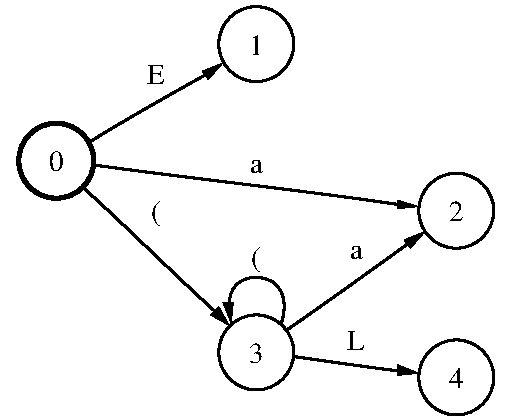
\includegraphics[height=2in]{figures/quiz2-lr}
\end{center}

The incomplete LR(0) action/goto table created from the automaton is shown below:
\begin{center}
\begin{tabular}{||l|c|c|c|c||c|c||}
\hline
   & (       & )     & a       & \$    & E      & L \\
\hline
\hline
 0 & shift 3 & error & shift 2 & error & goto 1 &     \\
\hline
 1 & error   & error & error   & accept &       &     \\
 \hline
 2 & reduce(2) & reduce(2) & reduce(2)   & reduce(2) &       &      \\
 \hline
 3 & shift  3 & & shift  2 &  &  goto 6     & goto 4     \\
   & reduce(4) & reduce(4) & reduce(4) & reduce(4) &       &    \\
 \hline
 4 &  error & shift 5 & error  &  error &       &      \\
 \hline
 5 &  &  &    &  &       &      \\
 \hline
 6 &  &  &    &  &       &      \\
 \hline
 7 &  &  &    &  &       &      \\
 \hline
 \hline
\end{tabular}
\end{center}

\bigskip

Your task for this question has four components:
\bigskip
\begin{xlist}
\ex{\label{lr1} Add the remaining three itemsets (use the numbers 5, 6, 7 for the new itemsets as indicated by entries in the action/goto table), and then
\begin{soln}
\[
\begin{array}{llcl}
5: & E & \rightarrow & ( L ) \ \bullet\ \\
&&& \\
6: & L  & \rightarrow & E \bullet\ L \\
& L  & \rightarrow & \epsilon\ \bullet\ \\
& L  & \rightarrow & \bullet\ E L \\
& E  & \rightarrow & \bullet\ a \\
& E  & \rightarrow & \bullet\ ( L ) \\
&&& \\
7: & L & \rightarrow & E L\ \bullet\  \\
\end{array}
\]
\end{soln}
}
\ex{\label{lr2} Complete the LR(0) automaton by adding the three new states including all the necessary transitions, and then
\begin{soln}
\begin{center}
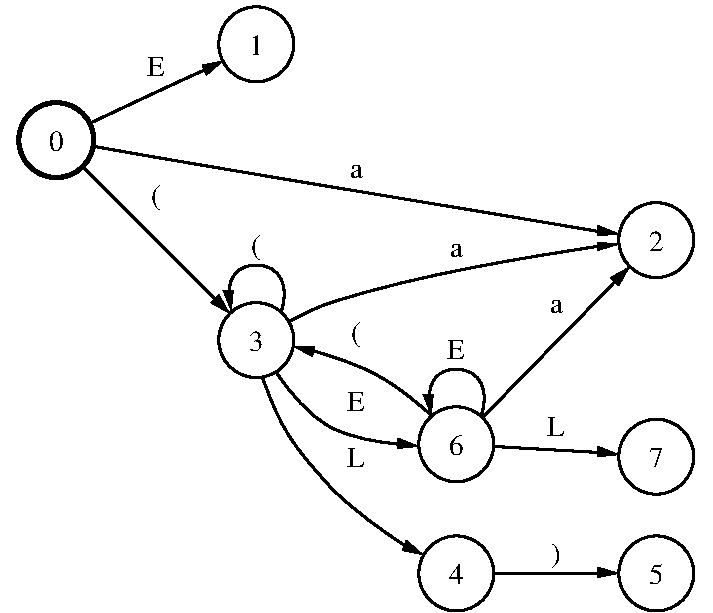
\includegraphics[width=4in]{figures/quiz2-lr-ans}
\end{center}
\end{soln}
}
\ex{\label{lr3} Complete the action/goto table entries (remember to indicate error entries), and finally
\begin{soln}
\begin{center}
\begin{tabular}{||l|c|c|c|c||c|c||}
\hline
  & (       & )     & a       & \$    & E      & L \\
\hline
\hline
0 & shift 3 & error & shift 2 & error & goto 1 &     \\
\hline
1 & error   & error & error   & accept &       &     \\
\hline
2 & reduce(2) & reduce(2) & reduce(2)   & reduce(2) &       &      \\
\hline
3 & shift  3 & & shift  2 &  &  goto 6     & goto 4     \\
  & reduce(4) & reduce(4) & reduce(4) & reduce(4) &       &    \\
\hline
4 &  error & shift 5 & error  &  error &       &      \\
\hline
5 & reduce(3) & reduce(3) & reduce(3)   & reduce(3) &       &      \\
\hline
6 & shift 3 & error & shift 2   & error &  goto 6   &  goto 7    \\
  & reduce(4) & reduce(4) & reduce(4) & reduce(4) &       &    \\
\hline
7 & reduce(5)  &reduce(5)  & reduce(5)   & reduce(5) &       &      \\
\hline
\hline
\end{tabular}
\end{center}
\end{soln}
}
\ex{\label{lr4} Indicate whether the grammar $G$ is a LR(0) grammar
\begin{soln} nope. conflicts all over the place. \end{soln}
}
\end{xlist}


\newpage

  \ex\label{cfg2}  Consider the following grammar $G$:
  \begin{eqnarray}
    S & \rightarrow & aSa \mid bSb \mid aa \mid bb \nonumber
  \end{eqnarray}
      
  \begin{xlist}
    {\ex Is the CFG $G$ an LL($1$) grammar? Provide a reason for your
    answer.
      \begin{soln}
        No. FIRST(aSa) intersected with FIRST(aa) is non-empty.
      \end{soln}
    }

    {\ex  Based on inspecting the set of possible viable prefixes for
      grammar $G$, is $G$ an LR(1) grammar? Provide an example viable
      prefix or a comparison between two candidate viable prefixes to
      support your answer.
      \begin{soln}
        No. While the grammar is unambiguous, consider the potential
        viable prefix $a^\ast b^\ast a aa a$ and the potential
        viable prefix $a^\ast b^\ast aa$ -- the same prefix can lead
        to a shift on $a$ or a reduce using $S \rightarrow aa$ on
        the handle $a^\ast b^\ast aa$. 
      \end{soln}
    }

    {\ex Consider a slightly modified version of grammar $G$. Let's
      call it $G'$:
      \begin{eqnarray}
        S & \rightarrow & aSa \mid bSb \mid \epsilon \nonumber
      \end{eqnarray}
      Does this modified grammar $G'$ generate the same language as
      the original grammar $G$? Provide a reason for your answer.
      \begin{soln}
        No. It now includes $\epsilon$ in the language.
      \end{soln}
    }
    
    {\ex  Is $G'$ an LL($1$) grammar? Provide a reason for your answer.
      \begin{soln}
        No, it is still not an LL($1$) grammar because the intersection
        of FIRST($aSa$) and FOLLOW($S$) = $\{ a, b, \$ \}$ is
        non-empty.
      \end{soln}
    }
    {\ex  Consider a slightly modified version of grammar $G$. Let's
      call it $G'$:
      \begin{eqnarray}
        S & \rightarrow & aSa \mid bSb \mid \epsilon \nonumber
      \end{eqnarray}
     Is $G'$ an LL($1$) grammar? Provide a reason for your answer.
      \begin{soln}
        No, it is still not an LL($1$) grammar because the intersection
        of FIRST($aSa$) and FOLLOW($S$) = $\{ a, b, \$ \}$ is
        non-empty.
      \end{soln}
    }
  \end{xlist}

\newpage
  \ex\label{lrgram}  For each grammar below indicate whether or
  not it is an LL($1$) grammar, an LR($0$) grammar, an SLR($1$)
  grammar and/or an LR($1$) grammar. \textit{For each grammar you have to
  provide four distinct yes/no answers}. 
  Provide a short reason for each yes or no answer. Note that
  each grammar below has production rules separated by commas.

  \begin{xlist}

    {\ex \( S \rightarrow A \mid B\ ,\ A \rightarrow c \mid dAd\ ,\ B
      \rightarrow c \mid dBd \) 
      \begin{soln}
        No to all. Ambiguous.
      \end{soln}
    }

    {\ex \( S \rightarrow A \mid B\ ,\ A \rightarrow c \mid dAd\ ,\ B
      \rightarrow e \mid dBd \) 
      \begin{soln}
        Not LL($1$), FIRST(A) $\cap$ FIRST(B) is not disjoint. Is LR(0)
        because the only case to where a conflict might occur is when
        items $S \rightarrow \bullet A$ and $S \rightarrow \bullet B$ predict
        two items: $A \rightarrow \bullet d A d$ and $B \rightarrow
        \bullet d B d$, but the successor on $A$ and $B$ ensure that
        item $A \rightarrow d A d \bullet$ has to be in a different state
        from $B \rightarrow d B d \bullet$. Since grammar is LR(0) it 
        is also SLR(1) and LR(1).
      \end{soln}
    }

    {\ex \( S \rightarrow aA \mid bB\ ,\ A \rightarrow c \mid dAd\ ,\
      B \rightarrow c \mid dBd \) 
      \begin{soln}
        Is LL($1$). FIRST($aA$) $\cap$ FIRST($bB$) is disjoint. Is
        LR(0) since the change in the grammar from the previous
        question cannot introduce any new conflicts in the LR(0)
        table and therefore the grammar is SLR(1) and also LR(1).
      \end{soln}
    }

    {\ex \( S \rightarrow AaAb \mid BbBa\ ,\ A \rightarrow \epsilon\
      ,\ B \rightarrow \epsilon \) 
      \begin{soln}
        Is LL($1$) because FIRST($AaAb$) $\cap$ FIRST($BbBa$) is
        disjoint, but not SLR(1) as FOLLOW(A) $\cap$ FOLLOW(B) is not
        disjoint. Since grammar is not SLR(1) it is also not LR(0).
        Grammar is LR(1) because the LR(1) items
        $[ A \rightarrow \epsilon \bullet, a]$ and 
        $[ B \rightarrow \epsilon \bullet, b]$
        which occur in the same itemset have distinct lookahead
        due to the LR(1) closure condition. The successor on $A$
        and $B$ ensures that the two rules with $S$ as left-hand
        side will appear in different itemsets and therefore no
        other conflicts can occur.
      \end{soln}
    }

  \end{xlist}


\newpage
\begin{comment}
 \ex\label{infer} The expression \texttt{g(g)} on line 7 of the C
 program listed below is the application of a function to itself. The
 declaration on line 3 clearly gives the type \textit{integer} as the
 range type for \texttt{g}, but the types of the arguments of
 \texttt{g} are not specified.

{\small
 \begin{verbatim}
      1  #include <stdio.h>

      2  int f(int g(), int n)
      3  {
      4    if (n == 0) return(1);
      5    else return(n * g(g, n-1));
      6  }

      7  int main()
      8  {
      9    int n=5;
     10    printf("input=%d\n", n);
     11    printf("output=%d\n", f(f,n) );
     12  }
 \end{verbatim}
}
 \begin{xlist}

 {\ex Provide the output when the above C program is executed.

 \begin{soln} 120 \end{soln}

 }

 {\ex What familiar mathematical function is computed by the above C
 program.

 \begin{soln} $n!$ \end{soln}

 }

 {\ex What is the type of \texttt{g}.

 \begin{soln} \texttt{g} has a recursive type $\alpha = \alpha \times
 \textit{integer} \rightarrow \textit{integer}$ \end{soln}

 }

 {\ex The following syntax-directed definition does type inference. The
   synthesized attribute {\it type} is used to carry the type
   information.

 \begin{center}
 \begin{tabular}{|ll|}
 \hline
 \hline
 Rules & Syntax-directed definition\\
 \hline
 \hline
 $E \rightarrow E\ (\ E\ )$ & \textit{unify}( 1.type , 3.type
 $\rightarrow \alpha_i$ ) \\
 & where $\alpha_i$ is a new type variable (unused so far) \\
 & 0.type := $\alpha_i$ \\
 \hline
 $E \rightarrow E\ ,\ E$ & 0.type := 1.type $\times$ 3.type \\
 \hline
 $E \rightarrow \textbf{token}$ & 0.type := 1.type \\
 \hline
 \hline
 \end{tabular}
 \end{center}

 Using the above syntax-directed definition draw an annotated parse
 tree for the program fragment:
{\small
 \begin{verbatim}
 times(3 , g(g , 2))
 \end{verbatim} 
}
 You are given the following type information for the tokens:

 \begin{tabular}{rcl}
 {\tt 3} & : & {\it integer} \\
 {\tt 2} & : & {\it integer} \\
 {\tt times} & : & {\it integer} $\times$ {\it integer} $\rightarrow$
 {\it integer} \\
 {\tt g} & : & $\alpha$
 \end{tabular}

 The annotated parse tree should have a value for the attribute {\it
 type} after all the unify operations have been completed for every
 non-terminal node in the tree.

\begin{soln}
{\small
\begin{verbatim}
(E : alpha_2 = int
            ==> unify(int x int -> int, int x alpha_1 -> alpha_2),
                side-effect: alpha_1 = int, alpha_2 = int
  (E times) : int x int -> int
  \(
  (E : int x alpha_1
    (E 3) : int
    ,
    (E : alpha_1  
                ==> unify(alpha, alpha x int -> alpha_1), 
                    side-effect: alpha = alpha x int -> alpha_1
      (E g) : alpha
      \(
      (E : alpha x int
        (E g) : alpha
        ,
        (E 2)) : int
      \)))
  \))
\end{verbatim}
}
\end{soln}
 }

 \end{xlist}
  \end{comment}
  
\newpage

\ex\label{opt} Consider the following three-address code (TAC) program:

  \begin{verbatim}
    i := m - 1
    j := n
    t1 := 4 * n
    v := A[ t1 ]
L1: i := i + 1
    t2 := 4 * i
    t3 := A[ t2 ]
    if t3 < v goto L1
L2: j := j - 1
    t4 := 4 * j
    t5 := A[ t4 ]
    if t5 > v goto L2
    if i >= j goto L3
    t6 := 4 * i
    x := A[ t6 ]
    t7 := 4 * i
    t8 := 4 * j
    t9 := A[ t8 ]
    A[ t7 ] := t9
    t10 := 4 * j
    A[ t10 ] := x
    goto L1
L3: t11 := 4 * i
    x := A[ t11 ]
    t12 := 4 * i
    t13 := 4 * n
    t14 := A[ t13 ]
    A[ t12 ] := t14
    t15 := 4 * n
    A[ t15 ] := x
  \end{verbatim}

  \begin{xlist}

    {\ex\label{flowgraph} Construct the control flowgraph for the above TAC program.
    \begin{soln}
	
	\begin{minipage}[t]{1.5in}
	{\small
    \begin{verbatim}
B1:    
  i = m-1
  j = n
  t1 = 4 * n
  v = A[t1]

B2: 
  i = i+1
  t2 = 4 * i
  t3 = A[t2]
  if t3<v goto B2

B3:
  j = j-1
  t4 = 4*j
  t5 = A[t4]
  if t5>v goto B3
    \end{verbatim}
    }
    \end{minipage}
	\begin{minipage}[t]{1.5in}
    {\small
    \begin{verbatim}
B4:
  if i>=j goto B6

B5:
  t6 = 4*i
  x = A[t6]
  t7 = 4*i
  t8 = 4*j
  t9 = A[t8]
  A[t7] = t9
  t10 = 4*j
  A[t10] = x
  goto B2      
    \end{verbatim}
    }
    \end{minipage}
	\begin{minipage}[t]{1.5in}
    {\small
    \begin{verbatim}
B6:
  t11 = 4*i
  x = A[t11]
  t12 = 4*i
  t13 = 4*n
  t14 = A[t13]
  A[t12] =  t14
  t15 = 4*n
  A[t15] = x
  
B1 --> B2 --> B3 --> B4 --> B5
B2 --> B2
B3 --> B3 
B5 --> B2
    \end{verbatim}
    }
    \end{minipage}
    \end{soln}
    }

    {\ex Perform {\em local} common subexpression elimination
      (i.e. only eliminate common subexpressions within each basic
      block) and provide the revised control flowgraph.
    \begin{soln}
	
	{\small
    \begin{verbatim}
B5:
  t6 = 4*i
  x = A[t6]
  t8 = 4*j
  t9 = A[t8]
  A[t6] = t9
  A[t8] = x
  goto B2

B6:
  t11 = 4*i
  x = A[t11]
  t13 = 4*n 
  t14 = A[t13]
  A[t11] = t14
  A[t13] = x
    \end{verbatim}
    }
    \end{soln}
    }

    {\ex The instruction {\tt t4 := 4*j} is repeatedly executed
    inside an inner loop (as can be seen in the control flow graph).
    Analyze the change in values in {\tt t4} and reduce the strength 
    of this instruction by replacing the multiplication operation
    with the cheaper operation (such as addition or subtraction). 
    In order to do this, you can add new instructions using expensive operations like
    multiplication as long as these instructions are added outside the inner loop.
    \begin{soln}

{\small
\begin{verbatim}
B1:
  i = m-1
  j = n
  t1 = 4*n
  v = A[t1]
  t4 = 4*j

B3:
  j = j-1
  t4 = t4-4
  t5 = A[t4]
  if t5>v goto B3
\end{verbatim}
}
    \end{soln}    
    }

\begin{comment}
  {\ex Do global common sub-expression elimination. Only provide the
  blocks that changed since question~(\ref{flowgraph}).
  \begin{soln}
  
	\begin{minipage}[t]{1.5in}
	{\small
    \begin{verbatim}
B1:    
  i = m-1
  j = n
  t1 = 4 * n
  v = A[t1]

B2: 
  i = i+1
  t2 = 4 * i
  t3 = A[t2]
  if t3<v goto B2

B3:
  j = j-1
  t4 = 4 * j
  t5 = A[t4]
  if t5>v goto B3
    \end{verbatim}
    }
    \end{minipage}
	\begin{minipage}[t]{1.5in}
    {\small
    \begin{verbatim}
B4:
  if i>=j goto B6

B5:
  x = t3
  A[t2] = t5
  A[t4] = x
  goto B2
    \end{verbatim}
    }
    \end{minipage}
	\begin{minipage}[t]{1.5in}
    {\small
    \begin{verbatim}
B6:
  x = t3
  t14 = A[t1]
  A[t2] = t14
  A[t1] = x
  
B1 --> B2 --> B3 --> B4 --> B5
B2 --> B2
B3 --> B3 
B5 --> B2
    \end{verbatim}
    }
    \end{minipage}
  \end{soln}
\end{comment}

  {\ex\label{ssa} For the following flowgraph construct the flowgraph
  in minimal Static Single Assignment (SSA) form. A {\em minimal} SSA form
  has no redundant static variable definitions.

  \begin{center}
  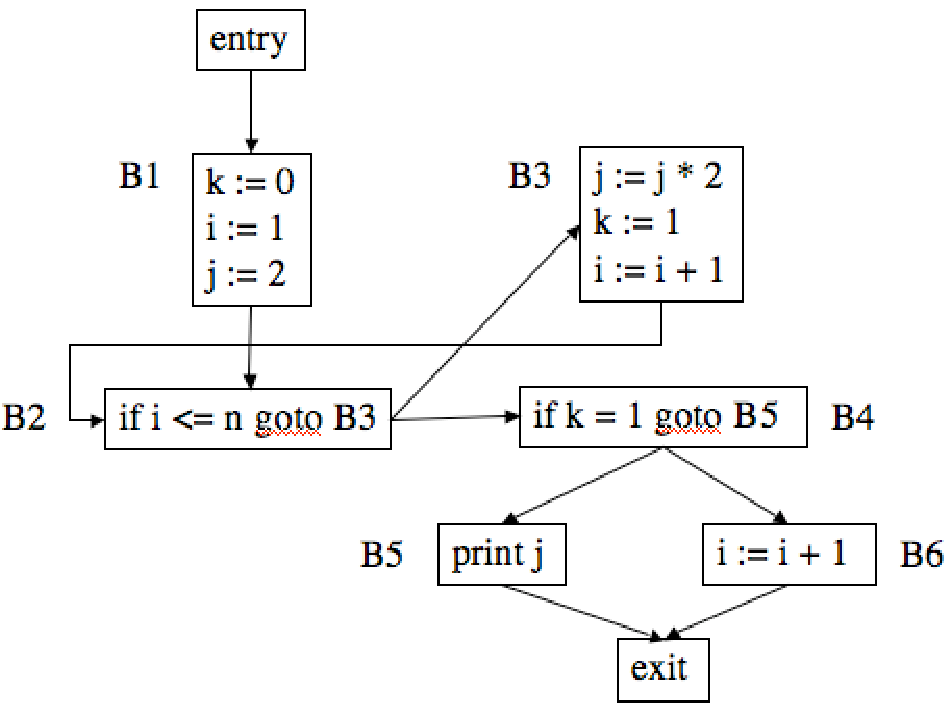
\includegraphics[height=3in]{figures/ssa-ex1-input}
  \end{center}

  \begin{soln}
  \begin{center}
  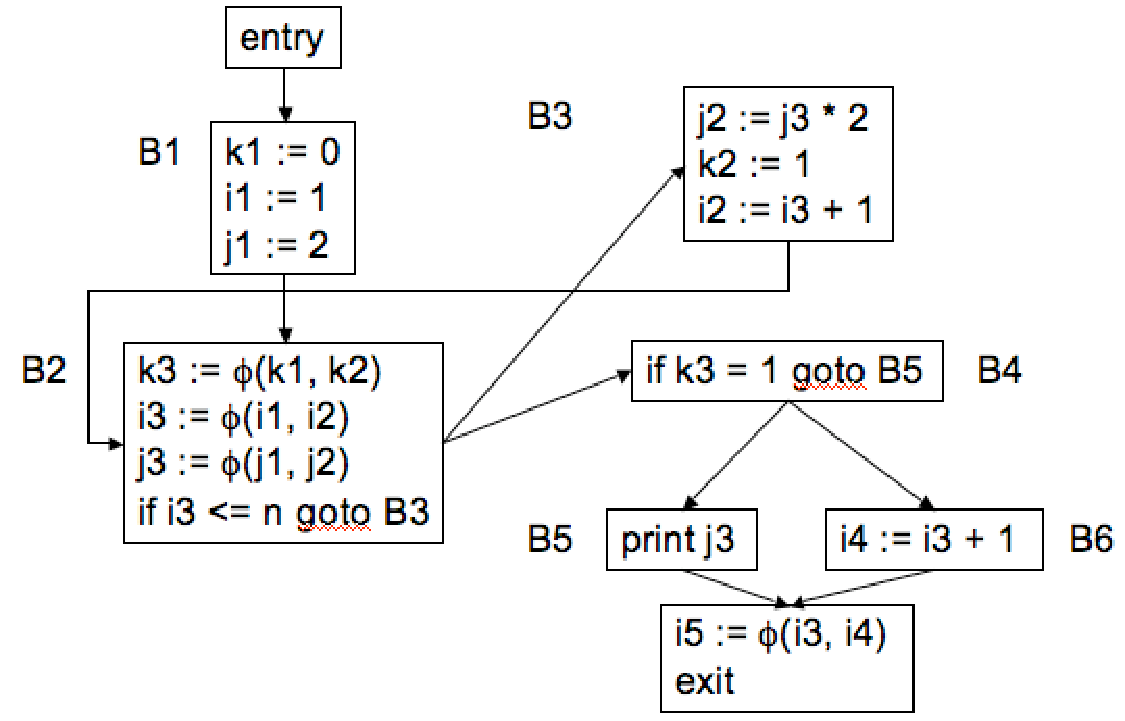
\includegraphics[height=2.5in]{figures/ssa-ex1-output}
  \end{center}
  \end{soln}
  }
  
  \end{xlist}

  \bigskip

 
\end{exe} 
\end{document}

